\documentclass[sigplan, anonymous, review]{acmart}

\usepackage{booktabs} % For formal tables


% Copyright
%\setcopyright{none}
%\setcopyright{acmcopyright}
%\setcopyright{acmlicensed}
\setcopyright{rightsretained}
%\setcopyright{usgov}
%\setcopyright{usgovmixed}
%\setcopyright{cagov}
%\setcopyright{cagovmixed}


% DOI
\acmDOI{10.475/123_4}

% ISBN
\acmISBN{123-4567-24-567/08/06}

%Conference
\acmConference[WOODSTOCK'97]{ACM Woodstock conference}{July 1997}{El
  Paso, Texas USA}
\acmYear{1997}
\copyrightyear{2016}

\acmPrice{15.00}

%\acmBadgeL[http://ctuning.org/ae/ppopp2016.html]{ae-logo}
%\acmBadgeR[http://ctuning.org/ae/ppopp2016.html]{ae-logo}

% Submission ID
\acmSubmissionID{123-A56-BU3}


\begin{document}
\title{Software Restoration of Legacy-Parallel Pthreads Parallel Applications}
\titlenote{Produces the permission block, and
  copyright information}
\subtitle{Extended Abstract}
%\subtitlenote{The full version of the author's guide is available as
  %\texttt{acmart.pdf} document}

\author{Discovery St Andrews People}
\authornote{Some note about Discovery People}
\orcid{1234-5678-9012}
\affiliation{%
  \institution{Institute for Clarity in Documentation}
  \streetaddress{P.O. Box 1212}
  \city{Dublin}
  \state{Ohio}
  \postcode{43017-6221}
}
\email{trovato@corporation.com}

%\author{G.K.M. Tobin}
%\authornote{The secretary disavows any knowledge of this author's actions.}
%\affiliation{%
%  \institution{Institute for Clarity in Documentation}
%  \streetaddress{P.O. Box 1212}
%  \city{Dublin}
%  \state{Ohio}
%  \postcode{43017-6221}
%}
%\email{webmaster@marysville-ohio.com}

%% \author{Aparna Patel}
%% \affiliation{%
%%  \institution{Rajiv Gandhi University}
%%  \streetaddress{Rono-Hills}
%%  \city{Doimukh}
%%  \state{Arunachal Pradesh}
%%  \country{India}}
%% \author{Huifen Chan}
%% \affiliation{%
%%   \institution{Tsinghua University}
%%   \streetaddress{30 Shuangqing Rd}
%%   \city{Haidian Qu}
%%   \state{Beijing Shi}
%%   \country{China}}

%% \author{Charles Palmer}
%% \affiliation{%
%%   \institution{Palmer Research Laboratories}
%%   \streetaddress{8600 Datapoint Drive}
%%   \city{San Antonio}
%%   \state{Texas}
%%   \postcode{78229}}
%% \email{cpalmer@prl.com}

%% \author{John Smith}
%% \affiliation{\institution{The Th{\o}rv{\"a}ld Group}}
%% \email{jsmith@affiliation.org}

%% \author{Julius P.~Kumquat}
%% \affiliation{\institution{The Kumquat Consortium}}
%% \email{jpkumquat@consortium.net}


% The default list of authors is too long for headers.
\renewcommand{\shortauthors}{Discovery et al.}



\begin{abstract}
  This paper describes pattern discovery mechanisms developed in the Discovery project.
\end{abstract}

%
% The code below should be generated by the tool at
% http://dl.acm.org/ccs.cfm
% Please copy and paste the code instead of the example below.
%
%\begin{CCSXML}
%<ccs2012>
% <concept>
%  <concept_id>10010520.10010553.10010562</concept_id>
%  <concept_desc>Computer systems organization~Embedded systems</concept_desc>
%  <concept_significance>500</concept_significance>
% </concept>
% <concept>
%  <concept_id>10010520.10010575.10010755</concept_id>
%  <concept_desc>Computer systems organization~Redundancy</concept_desc>
%  <concept_significance>300</concept_significance>
% </concept>
% <concept>
%  <concept_id>10010520.10010553.10010554</concept_id>
%  <concept_desc>Computer systems organization~Robotics</concept_desc>
%  <concept_significance>100</concept_significance>
% </concept>
% <concept>
%  <concept_id>10003033.10003083.10003095</concept_id>
%  <concept_desc>Networks~Network reliability</concept_desc>
%  <concept_significance>100</concept_significance>
% </concept>
%</ccs2012>
%\end{CCSXML}

%\ccsdesc[500]{Computer systems organization~Embedded systems}
%\ccsdesc[300]{Computer systems organization~Redundancy}
%\ccsdesc{Computer systems organization~Robotics}
%\ccsdesc[100]{Networks~Network reliability}


\keywords{ACM proceedings, \LaTeX, text tagging}

%\begin{teaserfigure}
%  \includegraphics[width=\textwidth]{sampleteaser}
%  \caption{This is a teaser}
%  \label{fig:teaser}
%\end{teaserfigure}


\maketitle

\section{Introduction}

\noindent
Parallel patterns are well established high-level parallel programming model for producing portable, maintainable, adaptive and efficient parallel code. They have been endorsed by some of the biggest IT companies, such as Intel and Microsfot, who have developed their own parallel pattern libraries (Intel TBB, Microsoft PPL etc.) A standard way of using these libraries is to start from the sequential code, identifying portions of the code that are amenable to parallelisation together with the exact parallel patternt to be applied, and then inserting calls to the identified patterns, after possibly restructuring the code to accommodate for parallelism. Sequential code gives the cleanest starting point for introduction of parallel patterns. There is, however, a large base of existing legacy code that was parallelised using lower-level, mostly ad-hoc parallelisation methods and libraries, such as pThreads. This code is usually tailored to one specific parallelisation and system architecture, with highly-specific and tuned data structures which prevent alternative (possibly more efficient parallelisations) or portability to different platforms. Also, code maintainance requires intricate knowledge about the system architecture and various low-level underlying mechanisms such as thread creation, synchronisation and scheduling. Introducing structured parallelism in form of parallel patterns into legacy-parallel code would bring numerous benefits in terms of maintainability and adaptivity to different systems. This is, however, a daunting task due to various factors, such as incompatibility between different threading libraries, high specialisation and tuning of the legacy code, usage of very specific data structures etc.


This paper presents a novel mechanism of \emph{software restoration}. Software restoration is removal of (undesirable) parallelism from the legacy-parallel code and elimination of the auxilary parallelism-specific data structures from it. The goal of restoration is to put the code in clean shape where structured parallelisation using parallel patterns can be applied. Software restoration is based on program analysis and software refactoring techniques. It is a semi-automated method that guide the programmer through the whole process of i) removing constructs to create and manage parallel threads; and, ii) removing the parallelisation-specific data structures that may present obstacle in discovery and introduction of structured parallelism. We evaluate our approach on a number of parallel applications, parallelised using pThreads library. We demonstrate that we are able to restructure the code and obtain the clean version onto which pattern discovery tools, and further pattern introduction/tuning refactoring can be applied to obtain efficient, portable and maintainable parallel code.

\begin{figure}
  \begin{center}
    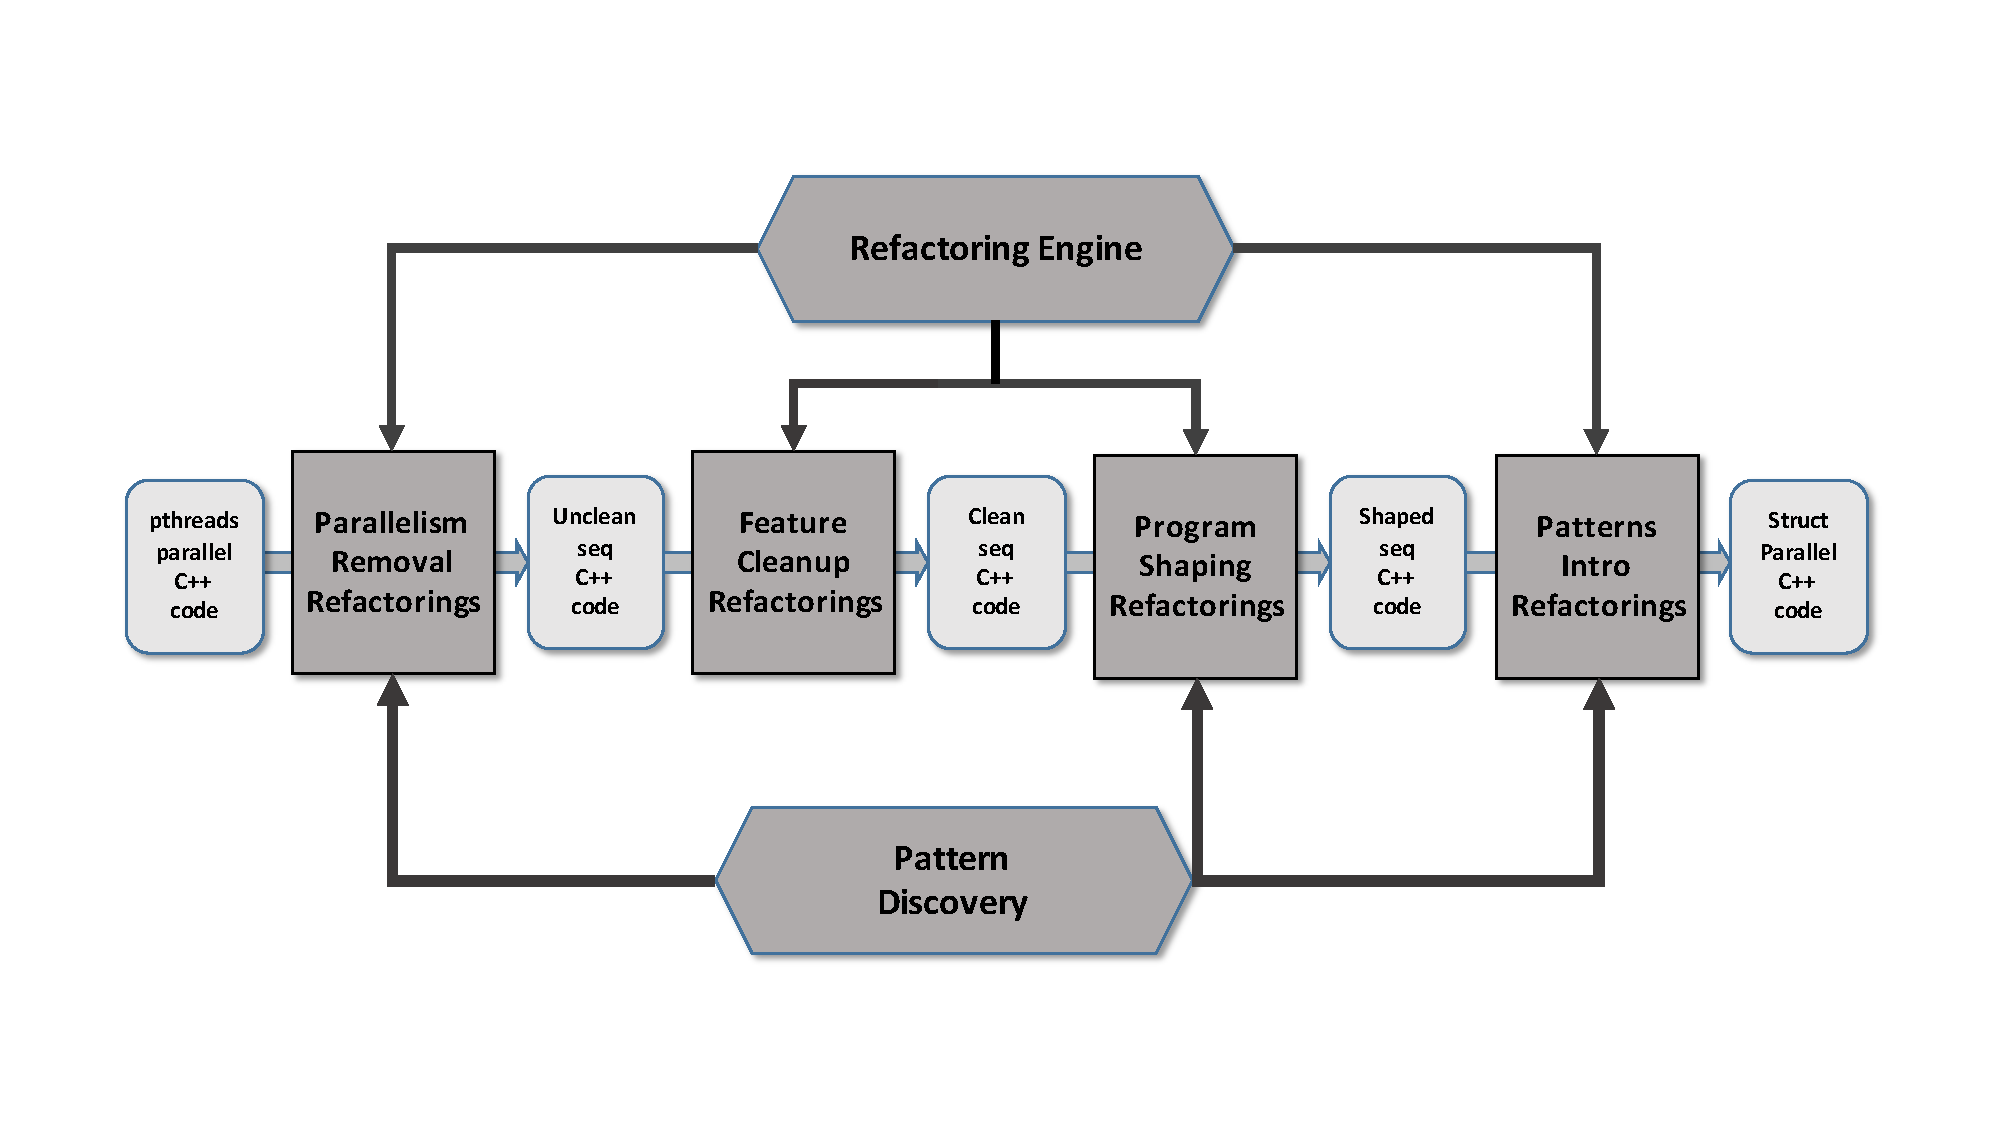
\includegraphics[width=0.5\textwidth]{SoftwareRestoration.pdf}
  \end{center}
  \vspace{-0.5cm}
  \caption{Software Restoration Process}
  \label{fig:SoftRest}

\end{figure}

%\input{samplebody-conf}

\bibliographystyle{ACM-Reference-Format}
%\bibliography{sample-bibliography}

\end{document}
